\chapter{Adversarial Examples Taxonomy}

This chapter focuses on Adversarial Crafting and how these examples can be used to exploit some of the Deep Neural Networks caveats seen in the last chapter. Firstly the Fast Gradient Sign method will be explained along with some results. Secondly, a brief discussion on the empty pockets of space created by neural networks enabling such technique to create adversarial. Finally a discussion of the potential threats these pose to systems relying on machine learning algorithms to perform their tasks.


\section{Foundations}

Understanding why adversarial samples exists requires exploration of how learning models are built. The training data is a corpus of samples taken from an expected input distribution and are labeled accordingly to their desired class. For instance, sample data would be a large number of emails or a huge data set of images.

The integrity of deep learning systems is usually measured by how accurate the system is when performing a classification task. This metric is of paramount importance and, therefore, is a common target for techniques trying to exploit such algorithms vulnerabilities. Specifically, an adversary of a deep learning system seeks to provide an input X' that results in incorrect output classification. The degree of incorrectness in the prediction can vary and, therefore, impacts the classifier output in different ways.

Adversary drivers could be classified by four goals as discussed by Papernot(2016) \cite{papernot_thesis_2016}. Confidence reduction is the adversary potential to introduce class ambiguity by reducing classification confidence. For instance, an input predicted with 99\% of confidence could have this level reduced without affecting the actual output of the network. Misclassification, on the other hand, happens when a label of the model being previously correct is randomly changed to an incorrect output label, affecting the model output. Another different type of misclassification is to actually create perturbations using a specific target class, this method forces the model to predict towards the specific desired class. Finally, one could use the same class to create perturbations that makes the class looks less likely itself, moving the prediction outcome to the nearest class in the data space.

\section{Domain Shift}

Regardless of the technique, a machine learning model represents an approximation of the phenomena being modeled. In most cases the training data is unable to represent all possible input feature vectors and, therefore, can not fully capture a complete understanding of the target domain. A problem arises when the system can be exploited by providing samples that are not within the aforementioned input domain. They usually use information about the system to find where the model is inaccurate owing to missing items of the given training set.

Classification accuracy should be carefully measured when training a model. For instance, the accuracy value obtained from the training set is usually higher than the one obtained from the test set. This happens when the samples of the training can not cover the entire data distribution space and therefore the domain covered differs from the one on the test set. A poor performance on the test set means that the divergence of both distributions (training and test domains) is high. 

What adversaries do is to force the domain shift in a way that the model is unable to generalize well on test data. Since data in most circumstances can not cover the entire feature space, the real decision boundary of a classification model generally becomes more complex as the phenomenon becomes more nuanced and the feature and dimension space becomes larger. This complexity is exploited by adversaries through the use of the model error as a guideline for perturbing a sample.

\begin{figure}[!h]
\centering
	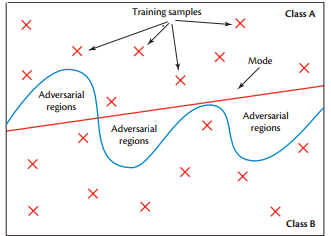
\includegraphics[scale=1.0]{adv_space.png}
\caption{Two Dimensional Representation of unexplored adversarial regions \cite{papernot_2017}}
\label{fig:adv_space}
\end{figure}

\section{Fast Gradient Sign Method - FGSM}

The Fast Gradient Signed method developed by Goodfellow et al. (2014) has been used as the foundation of many of the experiments in adversarial crafting. The results have led to the hypothesis that DNNs can possibly have linear behavior in very high dimensional space.  Most inputs were miss-classified not only on Goodfellow et. al \cite{goodfellow2014}  experiments but many other. This shows that adversarial examples are not hard to find. The method uses using gradient information to generate image noises that changes classification outputs.

$$ C(x + \delta)\approx C(x) + \delta * \nabla C$$

The equation aims to add noise that emphasizes the pixels in the image with the highest importance, so the resulting perturbation can likely lead to a misclassified result. By using the \textit(sign) function of the gradient, it is assured that the value will grow linearly with the number of the dimensions \cite{goodfellow2014}. The result of many small pixel changes is likely to generate an image with a wrong label in the network output.

$$ C(x + \delta)\approx C(x) + \delta * sign(\nabla C)$$

The Gradient Sign is an exploitation of the loss function in an optimization process so one can maximize any class score for a given input image. Since everything in a ConvNet is differentiable it is relatively straight forward to compute the gradient information of any specific class of the input domain. The process can be done by doing a forward pass on a network with the desired class output being set to 1 in the final layer, then the backpropagation retrieves the necessary changes on gradients that would make any image looks like the desired class. 

Billovits et al (2016) summarized four different categories of adversarials generated by FGSM. True Adversarial are those given a completely different label after being perturbed. Re-Focused adversarial is the method that changes the focus of an image by giving a classification of an object that used to have lower significance while keeping the original object presence. Conaturally Adversarial are those where the new output has some close relation to the miss-classified result (e.g. Dog and Cat). Finally, Benign adversarial happens when neural networks misses the top prediction of the original image but the adversarial example gets randomly classified correctly with high confidence \cite{billovits}.

\begin{figure}[!h]
\centering
	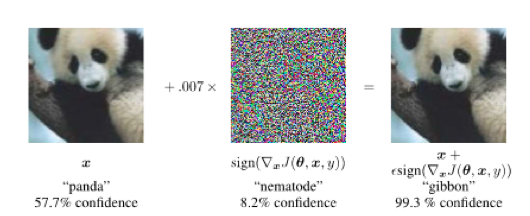
\includegraphics[scale=0.6]{panda.png}
\caption{Adversarial example crafting with fast gradient sign \cite{goodfellow2014}.}
\label{fig:fgsm_craft}
\end{figure}

\section{Iterative Gradient Sign Method - IGSM}

The method from the previous section shows that small perturbations can intentionally change classifiers class labels. Sometimes, more than one iteration of the Gradient Sign method is needed in order to have an image being incorrectly classified. By progressively apply small perturbations to an image one could achieve miss-classification of the desired sample that was not affected by one single iteration \cite{goodfellow2016}. 

\begin{figure}[!h]
	\centering
	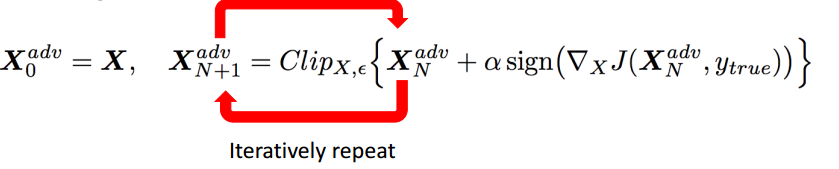
\includegraphics[scale=0.6]{iter_fgsm.png}
	\caption{Iterative FGSM Method \cite{goodfellow2016}.}
	\label{fig:iter_fgsm_craft}
\end{figure}
The extension of the fast method is reached by applying the gradient sign multiple times and clipping pixels that are not in the boundaries of the original image. Figure ~\ref{fig:iter_single_comp} shows the nature of perturbations of both methods. Since the FGSM applies a single batch of perturbation to the image, it needs a higher amount of noise at a time to be able to successfully generate an adversarial.
\begin{figure}[!h]
	\centering
	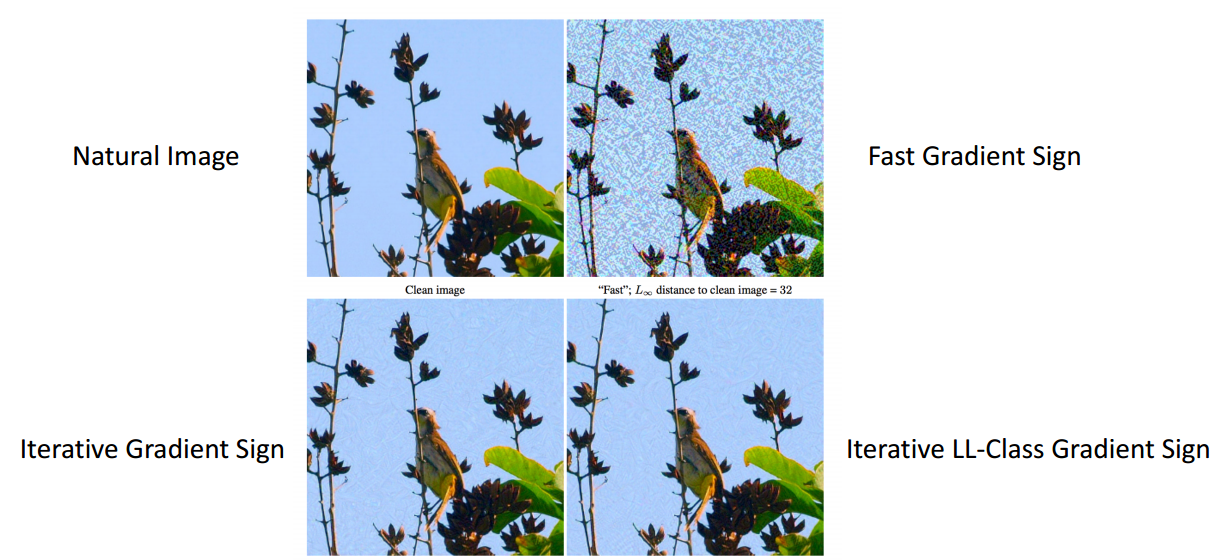
\includegraphics[scale=0.4]{iter_single.png}
	\caption{Visual Comparison of Gradients-based Methods \cite{goodfellow2016}.}
	\label{fig:iter_single_comp}
\end{figure}


\section{Ascent and Descent Perturbations}\label{sec:gsm}

Adding or subtracting noise from images would have generated different adversaries. By adding noise to an image, one would be making the gradient to go "uphill" and therefore moving away from the desired class, this results in an increase in value of the loss function and thus should be referred as the Ascent Method. On the other hand, when moving the opposite direction (down), one would be doing a process similar to the optimization of a loss function where we approach the minimum of a function and, thus, we get closer to the desired class, this approach is hereby known as the Descent Method. These two methods can be coupled with iterative methods or fast to take progressive/single steps towards a class directions. Some images/classes would be more robust to these perturbations and would, therefore, require more iterations.

$$ C(x + \delta)\approx C(x) + \delta * \nabla C - Ascent$$
$$ C(x + \delta)\approx C(x) - \delta * \nabla C - Descent$$